
\section{Essential Theory}
\subsection{Polynomial Representation}
A typical sequential circuit is composed as figure \ref{fig:sequential}. The combinational logic has primary input $x$, state
inputs $\{s_0, s_1, \dots, s_{k-1}\}$, primary output $z$ and state outputs $t_0, t_1, \dots, t_{k-1}$. State outputs
are latched into registers, which will be fed back to state inputs in next clock cycle.

\begin{figure}[hbt]
\begin{center}
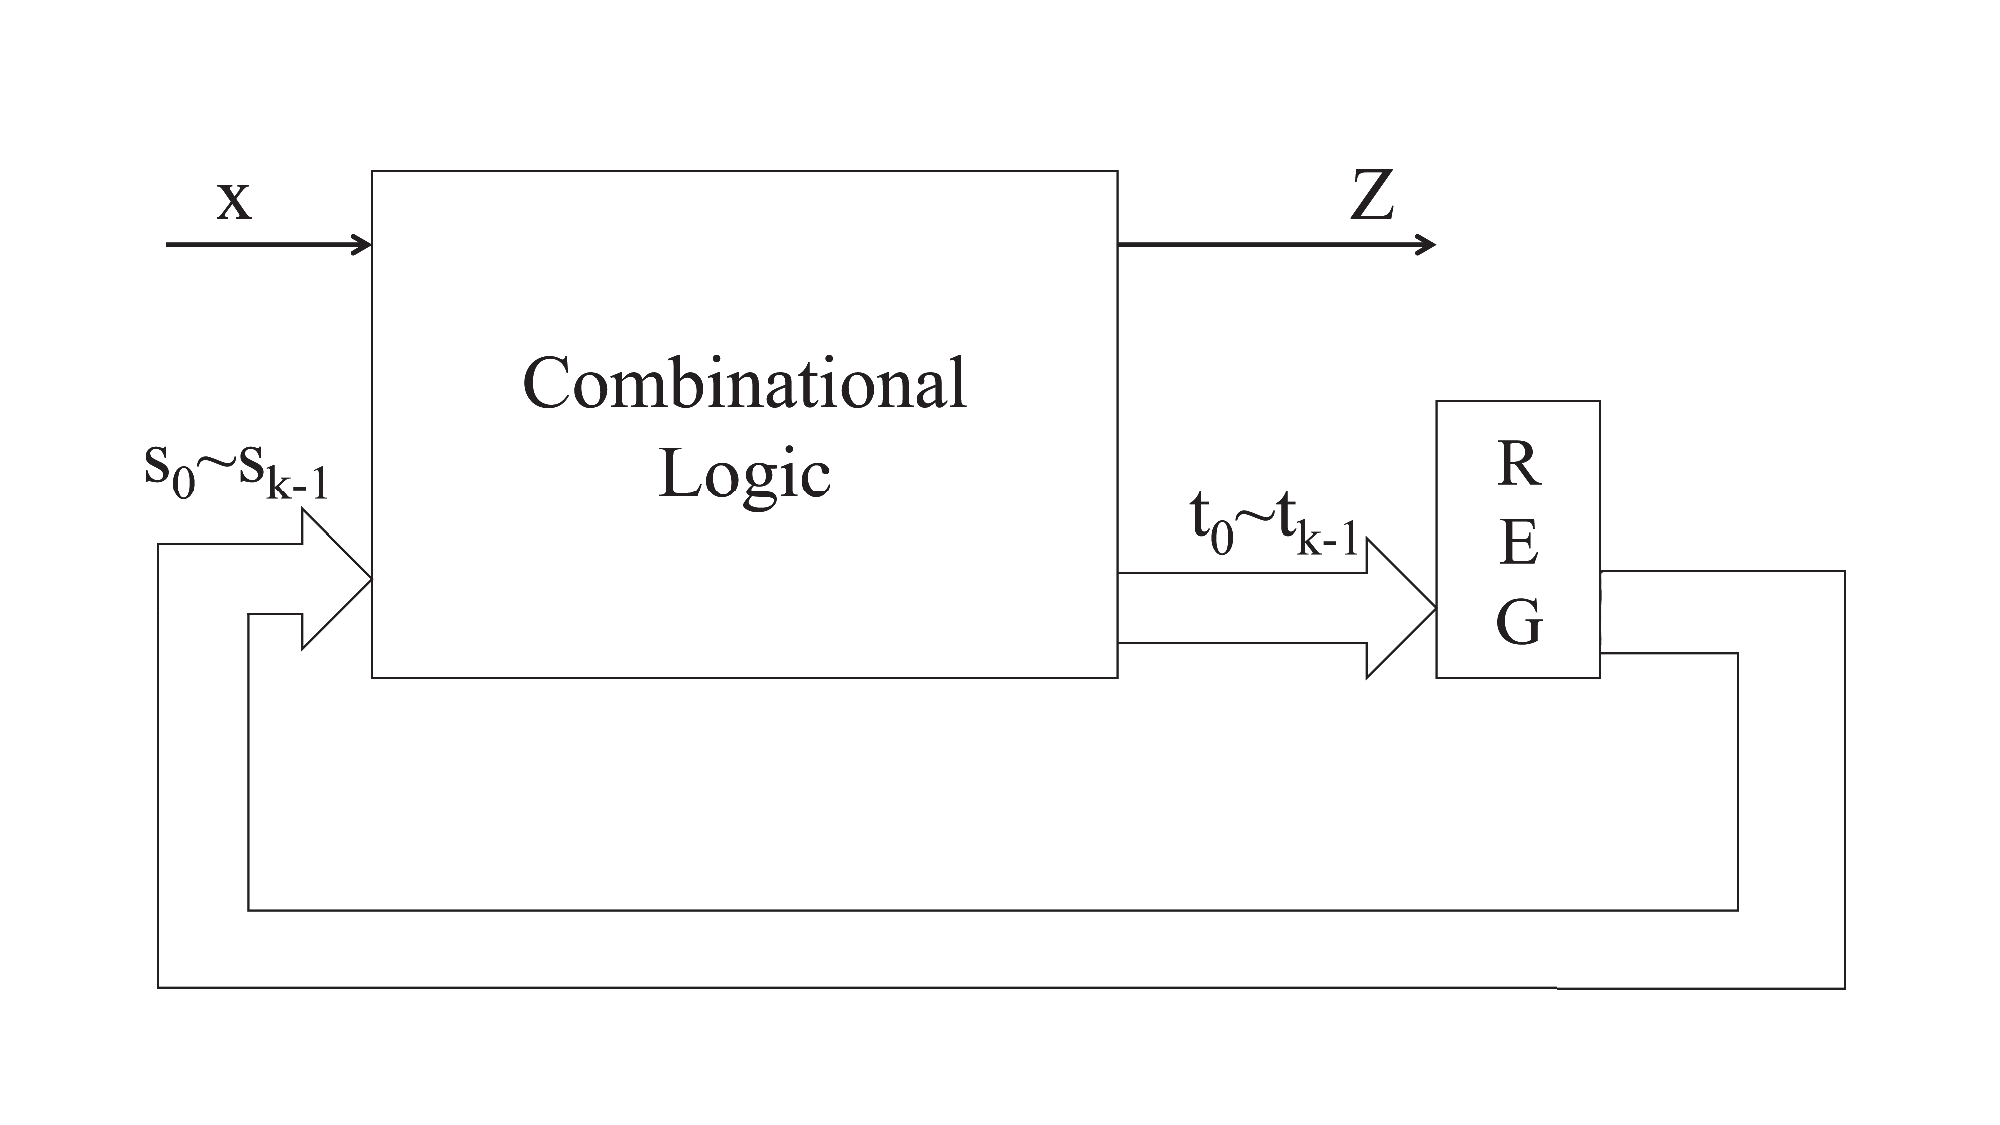
\includegraphics[width=3.5in]{./sequential_fig.eps}
\end{center}
\caption{A typical sequential circuit block view}
\label{fig:sequential}
\end{figure}


A transition function $\Delta$ is a Boolean function about state outputs and all inputs, i.e.
\begin{displaymath}
t_i = \Delta_i(x, s_0, s_1, \dots, s_{k-1})
\end{displaymath}
This constrain could also be written in the form of equation $polynomial = 0$:
\begin{displaymath}
t_i - \Delta_i(x, s_0, s_1, \dots, s_{k-1}) = 0
\end{displaymath}
Solution to this equation is limited within $\{0, 1\}$, which is set of all elements in Galois field $\mathbb{F}_2$.
Furthermore, there exists a one-to-one corresponding relation from Boolean space to Galois field on higher dimension: 
$\mathbb{B}^k \to \mathbb{F}_{2^k}$, which means it is possible to find a set of elements in $\mathbb{F}_{2^k}$ representing
all Boolean values every bit of a bit vector can take. In Galois field, a as \ref{table:booltogalois} shows.
\begin{table}[h]
\centering
\begin{tabular}{|c|c||c|c|} 
\hline
$a_3a_2a_1a_0$ & Polynomial     &$a_3a_2a_1a_0$ & Polynomial  \\
\hline
$0000$        & $0$           & $1000$  &$\alpha^3$\\
\hline
$0001$        & $1$           & $1001$  & $\alpha^3 + 1$\\
\hline
$0010$        &  $\alpha$       & $1010$ & $\alpha^3 + \alpha$  \\
\hline
$0011$        &  $\alpha + 1$   & $1011$ &  $\alpha^3+\alpha+1$\\
\hline
$0100$        &  $\alpha^2$     &  $1100$ &  $\alpha^3 + \alpha^2$\\
\hline
$0101$        & $\alpha^2 + 1$ & $1101$  & $\alpha^3+\alpha^2+1$\\
\hline
$0110$        &  $\alpha^2 + \alpha$ & $1110$ &  $\alpha^3+\alpha^2+\alpha$\\
\hline
$0111$        & $\alpha^2+\alpha+1$ & $1111$ & $\alpha^3+\alpha^2+\alpha+1$\\
\hline
\end{tabular}
\caption{Bit-vector, Exponential and Polynomial representation of
elements in  ${\mathbb{F}}_{2^4} = {\mathbb{F}}_2[x]
\pmod{x^4+x^3+1}$}\label{table:booltogalois}  
\end{table}
A word-level representation on state inputs/outputs can be attained through above correspondence. If the set of 
state inputs $\{s_0, s_1, \dots, s_{k-1}\}$ is denoted by $S$ taking values from $\mathbb{F}_{2^k}$, and
set of outputs $\{t_0, t_1, \dots, t_{k-1}\}$ is denoted by $T$, a word-level transition function can be written as
\begin{displaymath}
T - \Delta(x, S) = 0
\end{displaymath}
If $T - \Delta(x, S)$ is taken as a polynomial $f$, then $f \in \mathbb{F}_{2^k}[x]\ mod\ P(\alpha)$.
\subsection{Gr\"obner Basis Theory}
Gr\"obner basis is used to calculate desired results out of a set of polynomials.
If there exists multiple polynomials $\{f_1, f_2, \dots, f_r\}$ representing constrains on $T, x$ and $S$,
then all polynomials should simultaneously equal to $0$.
\begin{displaymath}
\left\{
  \begin{array}{lc}
  f_1 & = 0\\
  f_2 & = 0\\
  \dots & \ \\
  f_r & = 0
  \end{array} \right.
\end{displaymath}
Solution to these equations is set of values of $(T, x, S)$, which is called \textbf{Variety} of \textbf{ideal}
$I = \langle f_1, f_2, \dots, f_r\rangle $.

Calculate Reduced Gr\"obner Basis (RGB) from ideal $I$ with \textbf{elimination term order}, there exists a polynomial contains
only $T$, if the values of states input $S$ and primary input $x$ are given in the form of polynomials and included by $I$,
the values of $T$ can be computed.

Otherwise, if RGB calculation is manipulated under \textbf{abstraction term order}, there exists a polynomial in
the form of $T - \mathcal{F}(x, S)$ representing transition function. In next clock cycle, assign new state input $S'$ with $T$, the next
state can be computed again, result is polynomial $T' - \mathcal{F}(x', S')$. 

\subsection{Normal Basis Representation}

Let $\beta$ be an element in the Galois field $F_{2^n}$ constructed by primitive element $\alpha$ and minimal polynomial
$P(\alpha)$. Then a basis in the form $\{\beta, \beta^2, \beta^4, \beta^8, ... ,\beta^{2^{n-1}}\}$ is a
\emph{Normal Basis}; here $\beta$ is called \emph{Normal Element}.

For arithmetic operations in Galois fields, squaring and multiplication (with modulus) can be greatly simplified if 
normal basis representation is adopted to represent operands.
\begin{Example}
\label{ex:nb_sq}
Element squaring: In $F_{2^n}$, all coefficients which can be divided by 2 are reduced, so 
following equality holds for all field elements $a$ and $b$:
$$(a+b)^2 = a^2 + b^2$$ 
Apply this rule on element squaring of standard/polynomial basis:
\begin{align}
& (b_0\beta + b_1\beta^2 + b_2\beta^4 + \dots + b_{n-1}\beta^{2^{n-1}})^2 \nonumber\\
&= b_0^2\beta^2 + b_1^2\beta^4 + b_2^2\beta^8 + \dots + b_{n-1}^2\beta^{2^n} \nonumber\\
&= b_{n-1}^2\beta + b_0\beta^2 + b_1\beta^4 + \dots + b_{n-2}\beta^{2^{n-1}} \nonumber
\end{align}
using Fermat's little theorem $\beta^{2^n} = \beta$. This shows that squaring of field elements
represented by normal bases can be easily completed by operating a simple right-cyclic rotation.
\end{Example}

\begin{Example}
\label{ex:nb_multi}
Normal basis multiplication: There are 2 binary vectors representing operands of multiplication in normal
basis: $$A = (a_0, a_1, \dots, a_{n-1}),\ B = (b_0, b_1, \dots, b_{n-1})$$ 
the product is also written in normal basis representation: $$C = A*B = (c_0, c_1, \dots, c_{n-1})$$
Describe calculation procedure for the most significant digit of product with a function: 
$$c_{n-1} = f(a_0, a_1, \dots, a_{n-1}; b_0, b_1, \dots, b_{n-1})$$
Square both side: $C^2 = A^2*B^2$, i.e. the second significant digit 
$$c_{n-2} = f(a_{n-1}, a_0, a_1, \dots, a_{n-2}; b_{n-1}, b_0, b_1, \dots, b_{n-2})$$ 
By this method it is easy to get all digits of product $C$.
\end{Example}
  
\section{Algebraic Geometry Approach}
\subsection{State Space Traversal}

\begin{figure}[hbt]
\begin{center}
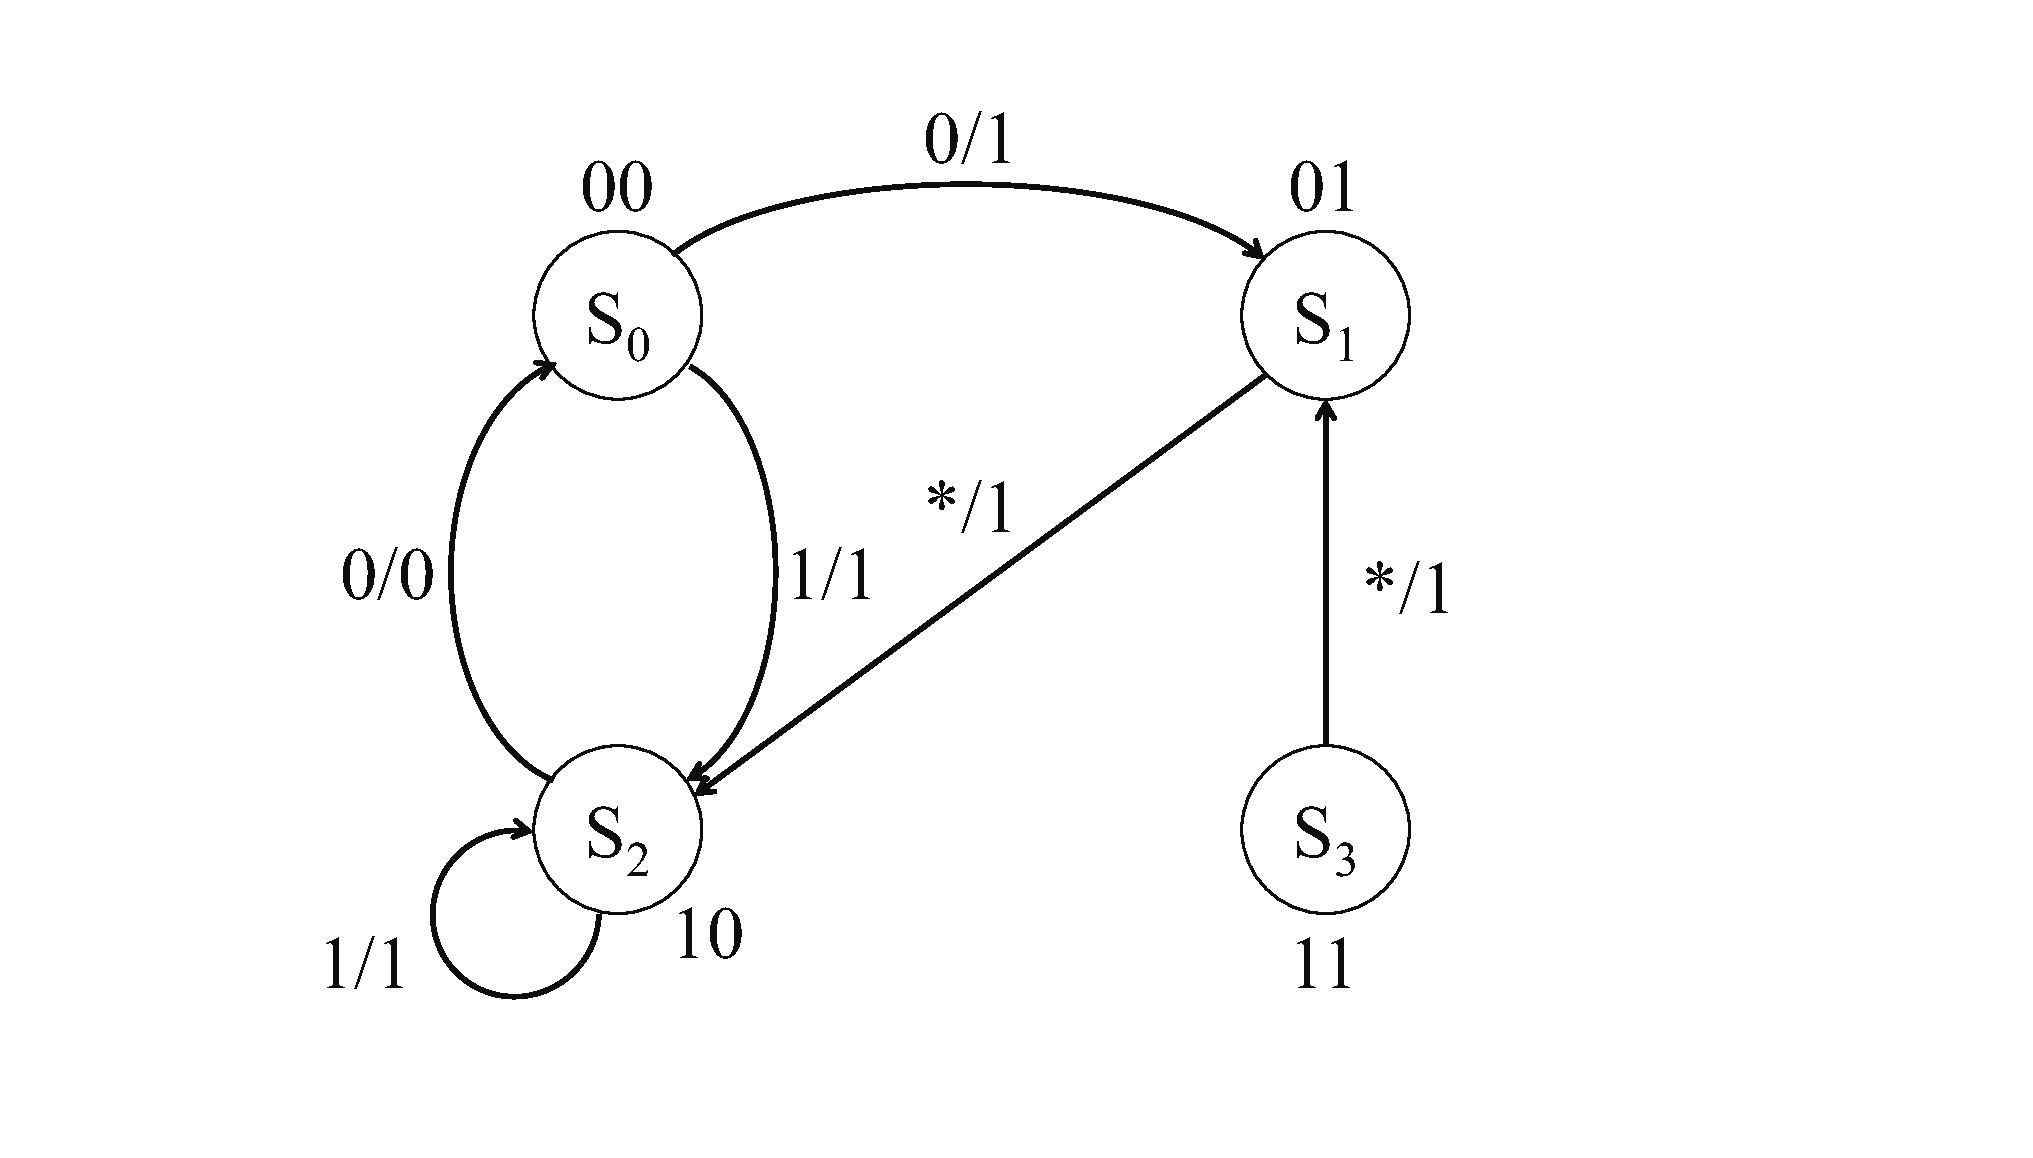
\includegraphics[scale=0.3]{./stg_fig.ps}
\end{center}
\caption{State transition graph of sample FSM}
\label{fig:stg}
\end{figure}

\begin{figure}[hbt]
\begin{center}
\includegraphics[width=3.5in]{./fsm_fig.eps}
\end{center}
\caption{Gate-level circuit of combinational logic block of sample FSM}
\label{fig:fsm}
\end{figure}

The first example is a mealy finite state machine (FSM). Gate-level circuits of combinational logic
is figure \ref{fig:fsm}, $x$ is primary input,
$\{s_0, s_1\}$ are state inputs, $Z$ is primary output and $\{t_0, t_1\}$ are state outputs.
Word-level state input is $S = s_0 + s_1\cdot\alpha$, output is $T = t_0 + t_1\cdot\alpha$. In Galois field
$\mathbb{F}_{2^2}$, bit-level variables $x, s_0, s_1, Z, t_0, t_1$ can take values from $\{0, 1\}$, while
word-level variables $S, T$ may take values from $\{0, 1, \alpha, 1 + \alpha\}$. State transition graph (STG)
showed in figure \ref{fig:stg} uses 2-bit Boolean vector to represent 4 states $\{S_0, S_1, S_2, S_3\}$, which
could be converted to elements in $\mathbb{F}_{2^2}$ similarly as table \ref{table:booltogalois} shows.

One important technique to check sequential equivalence is \textbf{state space traversal}. In this example,
Breath-First-Search (BFS) is employed for traversal, which can be described with following algorithm:

\begin{algorithm}[hbt]
\SetAlgoNoLine
 \KwIn{Transition functions $\Delta$, initial state $S^0$}

  $from^0 = reached = S^0$\;
  \Repeat{$new^i == 0$}
  {
  	$i \gets i + 1$\;
	$to^i \gets$Img$(\Delta, from^{i-1})$\;
	$new^i \gets to^i \cap \overline{reached}$\;
  	$reached \gets reached \cup new^i$\;
	$from^i \gets new^i$\;
  }
\Return{$reached$}
\caption {Breadth-first Traversal Algorithm}\label{alg:BFS}
\end{algorithm}

Our approach is implementing state space traversal by refined BFS algorithm combined with polynomial representation
and Gr\"obner basis theory. In practice, this example will show how to apply concepts and techniques from algebraic
geometry on each line of above BFS algorithm.

\subsection{States and Varieties of Ideal}

\begin{Theorem}
State variables $S, T$ and sets of states such as $from^i, to^i$ can always be represented as varieties of ideals.
\end{Theorem}
For example in Line 1 of BFS algorithm, assume initial state is $S_0$ in figure \ref{fig:stg}, then corresponding
polynomial $f = \mathcal{F}(S^0) = S^0 - 0$. Consider an ideal $I$ with only one generator $f$, its variety
$V(I) = \{\gamma\ |\ \gamma \in \mathbb{F}_{2^2}, \gamma = 0\}$, which equals to $\{0\}$, the only
valid value $S^0$ can take.

If an ideal contains multiple polynomial specifications, it is necessary to compute Gr\"obner basis with elimination term
order to get one polynomial only on desired variable. In first iteration of Line 4, $to^i$ has multiple specifications,
some of them are transition functions on bit-level:
\begin{displaymath}
\begin{array}{ll}
f_1:& t_0 - (\overline{x}\ and\ \overline{s_0}\ and\ \overline{s_1})\ or\ (s_0\ and\ s_1) \\
f_2:& t_1 - (\overline{s_0}\ and\ x)\ or\ (s_0\ and\ \overline{s_1})\
\end{array}
\end{displaymath}
And some are bits-to-word definitions fitting polynomial representation of elements in $\mathbb{F}_{2^2}$:
\begin{displaymath}
\begin{array}{ll}
f_3:& S - s_0 - s_1\alpha \\
f_4:& T - t_0 - t_1\alpha
\end{array}
\end{displaymath}
And an polynomial about initial state as mentioned above:
\begin{displaymath}
f_5:\  S
\end{displaymath}
And the rests are vanishing polynomials for every variable, bit-level and word level:
$f_6: x^2 - x; f_7: t_0^2 - t_0; f_8: t_1^2 - t_1; f_9: S^4 - S; f_{10}: s_0^2 - s_0;
f_{11}: s_1^2 - s_1; f_{12}: T^4 - T$

Transition equations here contains some Boolean operators, they can be re-written in terms of operations in Galois fields. 
In $\mathbb{F}_{2}$, let $TRUE = 1, FALSE = 0$, for either element $a$ in this field, considering $0 + 0 = 1 + 1 \equiv 0\ (mod\ 2)$
and $0 + 1 = 1 + 0 \equiv 1\ (mod\ 2)$, the inverse of $a$ is: $\overline{a} = 1 + a$. Similarly all Boolean operators
can be converted within $\mathbb{F}_{2}$, table \ref{table:booltogalois_op} gives part of them and their corresponding
operations in $\mathbb{F}_{2}$:
Also note that there is no specification on initial primary input $x$, in Gr\"obner basis approach this means $x$ is smoothed by
reversely using Shannon's expansion.
\begin{table}
\centering
\begin{tabular}{|c|c|} \hline
Boolean operator & operation in $\mathbb{F}_{2}$\\ \hline
$\overline{a}$ & $1 + a$\\ \hline
$a\ and\ b$ & $ab$\\ \hline
$a\ or\ b$ & $a + b + ab$\\ \hline
$a \oplus b$ & $a + b$\\
\hline\end{tabular}
\caption{Some Boolean operators and corresponding operations in $\mathbb{F}_{2}$}
\label{table:booltogalois_op}
\end{table}
Using elimination term order: $intermediate\ bit$-$level\ signals\ >\ bit$-$level\ primary\ inputs/outputs\ >\ S\ >\ T$, compute Gr\"obner basis for ideal
$J = \langle f_1, f_2, \dots, f_{12}\rangle $, the result will include one polynomial $f_T$ contains only variable $T$. In this example,
$f_T = T^2+(\alpha+1)T+\alpha$. This polynomial equals to $T^2-(\alpha+1)T+\alpha$ since coefficients of polynomial representation in $\mathbb{F}_{2^2}$ are
limited within $\mathbb{F}_{2}$, where $x \equiv -x\ (mod\ 2)$ for any element $x$ in the field. Solution to $f_T = 0$ is $T = 1\ or \ T = \alpha$, which shows that next
state the machine just reached is $\{S_1(01), S_2(10)\}$.

Continue to run this traversal algorithm, it will terminates with final reachable states $f_T = T^3+(\alpha+1)T^2+\alpha T$, its solution is $T=0\ or\ T=1\ or\ T=\alpha$,
which shows within total 4 states, state $S_3$ is unreachable from initial state $S_0$.

\subsection{Application of Algebraic Geometry}

There are some difficulties with polynomial representation when executing Line 5 and Line 6, it is necessary to explore
how \textbf{Union}, \textbf{Intersection} and \textbf{Complement Set} works in Galois field $\mathbb{F}_{2^k}$. Since
state set variables $from^i, to^i, reached$ all have single polynomial, consider an ideal $I$ with single generator $I = \langle f\rangle $.
Example: assume $I = \langle f\rangle  = \langle T^2 + (1+\alpha)\cdot T+\alpha\rangle $, its variety $V(I) = \{a\ |\ a \in \mathbb{F}_{2^2}\ and\ f(a) = 0\} = \{1, \alpha\}$.


\begin{figure*}[tb]
\begin{center}
\includegraphics[width=\textwidth]{./mySMPO.eps}
\end{center}
\caption{5-bit SMPO}
\label{fig:SMPO}
\end{figure*}

So it is reasonable to specify: union, intersection and complement set mentioned in this paper are all functions on \textbf{varieties}.
To better discuss this problem, introduce following concepts from algebraic geometry:
\begin{Definition}
\label{def:sum}
({\bf Sum of Ideals}) If $I$ and $J$ are ideals in $k[x_1, \dots, x_n]$, then the 
{\bf sum} of $I$ and $J$, denoted by $I + J$, is the set
  \begin{equation}
  I + J = \{f + g\ |\ f \in I \ and\  g \in J\}.
  \end{equation}
Furthermore, if $I = \langle f_1, \dots, f_r\rangle$ and 
$J = \langle g_1, \dots, g_s\rangle$, then 
$I + J = \langle f_1, \dots, f_r, g_1, \dots, g_s\rangle$.
\end{Definition}
\begin{Definition}
\label{def:prod}
({\bf Product of Ideals}) If $I$ and $J$ are ideals in $k[x_1, \dots, x_n]$, then the
{\bf product} of $I$ and $J$, denoted by $I \cdot J$, is defined to be the ideal generated 
by all polynomials $f \cdot g$ where $f \in I$ and $g \in J$. Furthermore, let
$I = \langle f_1, \dots, f_r\rangle$ and $J = \langle g_1, \dots, g_s\rangle$, then
  \begin{equation}
  I \cdot J = \langle f_ig_j\ |\ 1 \leq i \leq r, 1 \leq j \leq s\rangle .
  \end{equation}
\end{Definition}
\begin{Definition}
({\bf Quotient of Ideals}) If $I$ and $J$ are ideals in $k[x_1, \dots, x_n]$, then $I:J$
is the set
  \begin{equation}
  \{f \in k[x_1, \dots, x_n]\ |\ f\cdot g \in I, \forall g \in J\}
  \end{equation}
and is called the {\bf ideal quotient} of $I$ by $J$.
\end{Definition}
These concepts can lead the way to solution by adopting following theorems:
\begin{Theorem}
\label{thm:unionintersect}
If $I$ and $J$ are ideals in $k[x_1, \dots, x_n]$, then ${\bf V}(I + J) = {\bf V}(I)
\bigcap {\bf V}(J)$ and ${\bf V}(I \cdot J) = {\bf V}(I) \bigcup {\bf V}(J)$.
\end{Theorem}
\begin{Theorem}
\label{thm:quotient}
If $I, J$ are ideals with only one generator, then ${\bf V}(I:J) ={\bf V}(I) - {\bf V}(J)$.
\end{Theorem}
Proof to these theorems are referred to (that yellow book?) and (my write-up?).

For varieties intersection $\{1\}\bigcap\{1, \alpha\}$, calculate ideal sum $\langle T+1, T^2 + (1+\alpha)\cdot T+\alpha\rangle  = \langle T+1\rangle $,
its variety is $\{1\}$; for varieties union $\{1,\alpha\}\bigcup\{1+\alpha\}$, calculate
ideal product $\langle (T+1+\alpha)\cdot(T^2 + (1+\alpha)\cdot T+\alpha)\rangle  = \langle T^3 + 1\rangle $, its variety
is $\{1, \alpha, 1+\alpha\}$; for complement set of variety $\{1, \alpha\}$, the universal set is
the variety of ideal of vanishing polynomial $V(\langle T^4-T\rangle ) = \{0,1,\alpha,1+\alpha\}$,
so $\overline{V(\langle T^2 + (1+\alpha)\cdot T+\alpha\rangle )} = V(\langle T^4-T\rangle ) - V(\langle T^2 + (1+\alpha)\cdot T+\alpha\rangle )$,
which equals to $V(\langle T^4-T\rangle :\langle T^2 + (1+\alpha)\cdot T+\alpha\rangle ) = V(\langle T^2+(1+\alpha)\cdot T\rangle )$,
the result is $\{0,1+\alpha\}$.

From discussion above, the BFS traversal is completely implemented in Galois field.
If the initial input is $S_3$: $S + 1 + \alpha$, the final return value will be set of
reachable states: $T^4 + T$, i.e. the universal set, $\{S_0, S_1, S_2, S_3\}$. Modified algorithm could be
written in following interpretation:

\begin{algorithm}[hbt]
\SetAlgoNoLine
 \KwIn{Input-output circuit characteristic polynomial ideal $I_{ckt}$, initial state polynomial $\F(S)$}

  $from^0 = reached = \F(S)$\;
  \Repeat{$new^i == 1$}
  {
  	$i \gets i + 1$\;
	$to^i \gets$GB w/ elimination term order$<I_{ckt}, from^{i-1}>$\;
	$new^i \gets $generator of $<to^i> + (<T^4-T>:<reached>)$\;
  	$reached \gets $generator of $<reached> \cdot <new^i>$\;
	$from^i \gets new^i(S\setminus T)$\;
  }
\Return{$reached$}
\caption {Algebraic Geometry based Traversal Algorithm}\label{alg:modified}
\end{algorithm}

Here $from^i, to^i, new^i$ are all univariate polynomial about $S$ or $T$



\section{Functional Verification}
\subsection{Sequential Galois Arithmetic Multiplier}
Our experiment is to verify the function of a Galois field multiplier after certain clock cycles.
The following design is Sequential Multiplier with Parallel Output (SMPO),
a Normal Basis multiplier based on Massey-Omura algorithm. Inputs and outputs
are all 5-bit word taking value from ${\mathbb F}_{2^5}$. After loading operands
 A and B, setting all output latches to 0 and running for 5 iterations, the 
output should be $R = A\cdot B$ (mod $x^5 + x^2 + 1$).

Similarly, build elimination ideal for all gates/operations and induce
initial states of latches. However, instead of eliminating all variables
to one, this example adopts abstraction term order
and keeps the polynomial contains function between output and inputs.
Here the lex ordering is $\{all\ bit$-$level\ variables\} > R > \{A, B\}$, and objective
polynomial is $R + \mathcal{F}(A, B)$.

Apply this approach to calculate image in BFS traversal, but modify algorithm
\ref{alg:BFS} to make it adapt 5 steps reachable states enumeration.
The result is $R + AB$, which validates the function of this circuit.

\subsection{Gr\"obner basis based Approach}
\label{sec:SMPOexperiment}

For 5-bit normal basis multiplication, the $i$-th digit of product can be written as
\begin{align}
R_i &= b_ia_{i+1} + b_{i+1}(a_i + a_{i+3}) + b_{i+2}(a_{i+3} + a_{i+4}) \nonumber\\
&+ b_{i+3}(a_{i+1} + a_{i+2}) + b_{i+4}
(a_{i+2} + a_{i+4}),\ 0\leq i\leq 4 \nonumber
\end{align}
It is possible to calculate every conjunctive term in the product simultaneously within one clock cycle,
on distinct bits. 
Use cyclic similarity of above function, following executions are operated: 
\begin{Example}
Sequential Multiplier Protocol:
\begin{itemize}
\item \textbf{Initial}\ \ $R_0 = R_1 = R_2 = R_3 = R_4 = 0$
\item \textbf{Clock 1}\ \ $R_0 = a_1b_0, R_1 = b_2(a_1 + a_4), R_2 = b_4(a_0 + a_1), R_3 = b_1(a_4 + a_0), 
			R_4 = b_3(a_1 + a_3)$
\item \textbf{Clock 2}\ \ $R_0 = b_3(a_1 + a_3) + a_0b_4, R_1 = a_1b_0 + b_1(a_0 + a_3), R_2 = b_2(a_1 + a_4)
			+ b_3(a_4 + a_0), R_3 = b_4(a_0 + a_1) + b_0(a_3 + a_4), R_4 = b_1(a_4 + a_0) + b_2(a_0 + a_2)$
\item \textbf{$\dots$}
\item \textbf{Clock 5}\ \ $R_0 = c_0, R_1 = c_1, R_2 = c_2, R_3 = c_3, R_4 = c_4$, i.e. $R = A\cdot B$.
\end{itemize}
\end{Example}

In BFS algorithm, the \textbf{Image} function is implemented by constructing an elimination ideal then 
compute its Gr\"obner basis. 
\begin{Example}
\label{ex:SMPO}
For 5-bit SMPO, the ideal consists of (for the first clock cycle):

(a) {\bf Gate descriptions:}
$a_1+a_4+c_1, a_1+a_0+c_2, a_0+a_4+c_3, a_1+a_3+c_4,
		  a_1b_0+r_4+R_0, c_1b_2+r_0+R_1, c_2b_4+r_1+R_2, c_3b_1+r_2+R_3, c_4b_3+r_3+R_4;$
		  
(b) {\bf Word-level variables:}
$A+a_0\alpha^5+a_1\alpha^{10}+a_2\alpha^{20}+a_3\alpha^9+a_4\alpha^{18},
		  B+b_0\alpha^5+b_1\alpha^{10}+b_2\alpha^{20}+b_3\alpha^9+b_4\alpha^{18},
		  r+r_0\alpha^5+r_1\alpha^{10}+r_2\alpha^{20}+r_3\alpha^9+r_4\alpha^{18},
		  R+R_0\alpha^5+R_1\alpha^{10}+R_2\alpha^{20}+R_3\alpha^9+R_4\alpha^{18};$
		  
(c) {\bf Vanishing polynomials:}
		 $ a_0^2+a_0, a_1^2+a_1, a_2^2+a_2, a_3^2+a_3, a_4^2+a_4,
		  b_0^2+b_0, b_1^2+b_1, b_2^2+b_2, b_3^2+b_3, b_4^2+b_4,
		  r_0^2+r_0, r_1^2+r_1, r_2^2+r_2, r_3^2+r_3, r_4^2+r_4,
		  R_0^2+R_0, R_1^2+R_1, R_2^2+R_2, R_3^2+R_3, R_4^2+R_4,
		  c_1^2+c_1, c_2^2+c_2, c_3^2+c_3, c_4^2+c_4,
		  A^{32}+A, B^{32}+B, r^{32}+r, R^{32}+R;$
		  
(d)	{\bf Feedback input:}	  $r_{in}$.

Polynomial $r_{in}$ equals to $from^{i-1}$ in Line 4, BFS algorithm. Under abstraction term ordering,
polynomial $to^i$ is assigned with a polynomial in result Gr\"obner basis which has the form $R + \mathcal{F}(A,B)$. 
Since all outputs are connected to feedback inputs
in SMPO, Line 5 and 6 will be neglected. Line 7 is finished by replace current output $R$ with previous 
output $r$. Initially $r_{in} = 0$.

In next clock cycle, $r_{in} = r + \mathcal{F}(A,B)$ updated from latest result; simultaneously operands
$A$ and $B$ have been cyclically shifted, so gate descriptions in (a) should be modified accordingly. The 
loop is operated for 5 times, result from the last step's Gr\"obner basis should be polynomial $R + AB$.
\end{Example}

This experiment can be repeated on $n$-bits SMPO after running for $n$ clock cycles.

\section{Fast Gr\"obner basis computation}
\subsection{Refined abstraction term order (RATO)}
A lexicographic order constrained by following relation $>_{r}$: "circuit variables ordered reverse topologically" $>$ 
"designated word-level output" $>$ "word-level inputs" is called the \emph{Refined Abstraction Term Order (RATO)}.

In Buchberger's algorithm, the specification polynomial (Spoly) for each pair is calculated. In RATO, most polynomials
have relatively prime leading terms/monomials (which means $Spoly \xrightarrow{J+J_0}_{+} 0$) except one pair:
word-level polynomial corresponding to outputs and its leading bit-level variable's gate description polynomial.
Its remainder $r$ lets following lemma hold:

\begin{Lemma}
\label{lem:1}
$r$ will only contain primary inputs (bit-level and word-level) and word-level output; furthermore, there will be one and
only one term containing word-level output whose monomial is word-level output itself rather than higher order form.
\end{Lemma}

\begin{proof}
First proposition is easy to prove by contradiction. Second part, the candidate pair of polynomials only have one term of
single word-level output variable (say it is $R$) and this term is the last term under RATO, which means there is only one term with
$R$ in Spoly. Meanwhile in other polynomials from $J+J_0$ there is no such term containing $R$, so this term will be
kept to remainder $r$, in first degree.
\end{proof}

\begin{Example}
The elimination ideal for 5-bit SMPO (Ex.\ref{ex:SMPO}) could be rewritten under RATO:
\begin{align}
&(R_0,R_1,R_2,R_3,R_4)>(r_0,r_1,r_2,r_3,r_4)\nonumber\\&>(c_1,c_2,c_3,c_4,b_0,b_1,b_2,b_3,b_4)\nonumber\\
&>(a_0,a_1,a_2,a_3,a_4)>R>r>(A,B)\nonumber
\end{align}
Thus the candidate pair is
$(f_w,f_g), f_w = R_0+r_4+b_0\cdot a_1, f_g =R_0\alpha^5+R_1\alpha^{10}+R_2\alpha^{20}+R_3\alpha^9+R_4\alpha^{18} + R$.
Result after reduction is:
\begin{align}
&Spoly(f_w,f_g) \xrightarrow{J+J_0}_{+}\nonumber\\
&r_1+(\alpha)r_2+(\alpha^4+\alpha^2)r_3+(\alpha^3+\alpha^2)r_4+(\alpha^3)b_1a_1\nonumber\\
+&(\alpha^4+\alpha^2)b_1a_2+(\alpha^3+\alpha+1)b_1a_3+(\alpha^3+\alpha)b_1a_4+(\alpha+1)b_1A\nonumber\\
+&(\alpha^4+\alpha^2+\alpha)b_2a_1+(\alpha^4+\alpha^3+\alpha^2+\alpha)b_2a_4+(\alpha^3+\alpha^2+1)b_3a_1\nonumber\\
+&(\alpha)b_3a_3+(\alpha^2+\alpha+1)b_4a_1+(\alpha+1)b_4a_2+(\alpha^4+\alpha^2)b_4a_3\nonumber\\
+&(\alpha^4+\alpha^3+\alpha+1)b_4a_4+(\alpha^3+1)b_4A+(\alpha^4+\alpha^3+\alpha^2+1)a_1B\nonumber\\
+&(\alpha^4+\alpha^3+\alpha^2+1)R\nonumber
\end{align}
The remainder satisfies Lemma \ref{lem:1}.
\end{Example}

\subsection{Bit-level Variable Substitution (BLVS)}
\label{sec:blvs}
The remainder from \emph{Spoly} contains some bit-level variables, and our objective is to get a polynomial contains only word-level variables
(such as $R+\mathcal{F}(A,B)$). One possible method is to rewrite bit-level variables in term of function on word-level
variables, i.e. $a_i = \mathcal{G}(A)$, then do substitution. A Gaussian-elimination-fashion approach could be applied to
compute corresponding $\mathcal{G}(A)$ efficiently.

\begin{Example}
{\bf Objective}:\ Abstract polynomial $a_i + \mathcal{G}_i(A)$ from $f_0: a_0\alpha^5+a_1\alpha^{10}+a_2\alpha^{20}+a_3\alpha^9+a_4\alpha^{18}+A$.

First, compute $f_0^2: a_0\alpha^{10}+a_1\alpha^{20}+a_2\alpha^{9}+a_3\alpha^{18}+a_4\alpha^{5}+A^2$. Apparently variable $a_0$ can be
eliminated by operation 
\begin{align}
f_1 =& f_0\times \alpha^5 + f_0^2: \nonumber\\
&a_1+(\alpha)a_2+(\alpha^4+\alpha^2)a_3+(\alpha^3+\alpha^2)a_4\nonumber\\
+&(\alpha^4+\alpha^3+\alpha^2+1)A^2+(\alpha^2+\alpha)A\nonumber
\end{align}
Recursively eliminate $a_1$ from $f_1$, $a_2$ from $f_2$, etc. The final polynomial $f_4$ has the form 
$a_4 + \mathcal{G}_4(A) = a_4+(\alpha^4+\alpha^3+\alpha)A^{16}+(\alpha^3+\alpha^2)A^8+(\alpha^4+1)A^4+(\alpha^2+1)A^2+(\alpha+1)A$. Recursively substitute
$\mathcal{G}_4(A)$ back to $f_3$, etc. The result is a set of polynomials
\begin{displaymath}
\{g_i\ | \ g_i: a_i + \mathcal{G}_i(A)\}
\end{displaymath}
\end{Example}
In this approach it is easy to get word-level variable representation for each bit-level primary inputs. By substitution, a new polynomial in the form $R+\mathcal{F}(A,B)$
could be attained.

\textit{Discussion}\ \ (a) This approach won't conduct to a result reducing to 0, because \emph{Spoly}'s remainder contains information from the whole system,
the substitution will result something new, i.e. an abstraction of the system; (b) The Gaussian-like approach is a pre-processing of a variable, and could be immediately reused
to other words with the same length; (c) For $n$-bits SMPO, the fast GB is very efficient: for each cycle, first compute a \emph{Spoly} in $O(1)$, then do multi-division by $O(n)$ polynomials
(unknown complexity, maybe lower if using F4-style reduction?), the substitution cost at most $O(n^3)$ time (assuming $O(1)$ for each term). In total repeat for $n$ cycles.
The complexity should be much lower compared to Buchberger's algorithm.
% The following two commands are all you need in the
% initial runs of your .tex file to
% produce the bibliography for the citations in your paper.
%\bibliographystyle{abbrv}
%\bibliography{seq_verif}  % sigproc.bib is the name of the Bibliography in this case
% You must have a proper ".bib" file
%  and remember to run:
% latex bibtex latex latex
% to resolve all references
%
